\documentclass{article}
\usepackage[utf8]{inputenc}
\usepackage[margin=1.2in]{geometry}
\usepackage[toc,page]{appendix}
\usepackage{url}
\usepackage{hyperref}
\usepackage{natbib}
\usepackage{graphicx}
\usepackage{placeins}
\usepackage{amssymb}
\usepackage{amsmath}
\usepackage{breakurl}

\def\UrlBreaks{\do\A\do\B\do\C\do\D\do\E\do\F\do\G\do\H\do\I\do\J\do\K\do\L\do\M\do\N\do\O\do\P\do\Q\do\R\do\S\do\T\do\U\do\V\do\W\do\X\do\Y\do\Z\do\[\do\\\do\]\do\^\do\_\do\`\do\a\do\b\do\c\do\d\do\e\do\f\do\g\do\h\do\i\do\j\do\k\do\l\do\m\do\n\do\o\do\p\do\q\do\r\do\s\do\t\do\u\do\v\do\w\do\x\do\y\do\z\do\0\do\1\do\2\do\3\do\4\do\5\do\6\do\7\do\8\do\9\do\.\do\@\do\\\do\/\do\!\do\_\do\|\do\;\do\>\do\]\do\)\do\,\do\?\do\'\do+\do\=\do\#}


\title{\textbf{Set up node-gyp-Node.js native addon build tool}}
\author{Wanni Xie\\
\emial{wx243@cam.ac.uk}}
% \emial {wx243@cam.ac.uk}
\date{August 2020}

\usepackage{natbib}
\usepackage{graphicx}

\begin{document}

\maketitle

Firstly, please check the official setting up instructions at: \url{https://github.com/nodejs/node-gyp}.
 
Pre-installation: 
\begin{itemize}
    \item Node.js v11
    \item Visual Studio Community 2019 or 2015 (select all workloads during the installation)
    \item Visual Studio build tool 2019 or 2015
\end{itemize}
Note: If python2.7 is already installed in the user’s computer, please uninstalled it at this point. It doesn’t matter that other python versions still exist.
 
\FloatBarrier
\begin{figure}[h!]
\centering
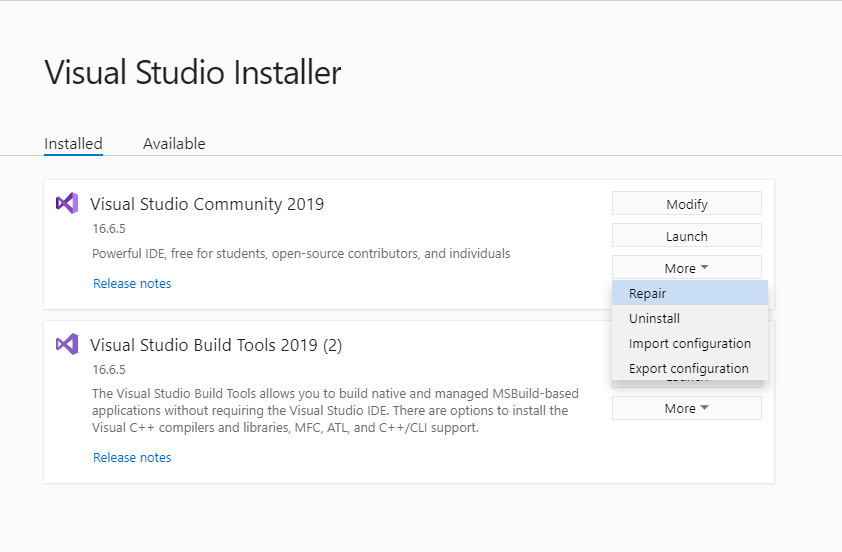
\includegraphics[scale=0.7]{installer.png}
\caption{The vs installer}
\label{fig:installer}
\end{figure}
\FloatBarrier

When all the installation finished, fellow the guidance of the installer or just restart the PC. It is better to avoid have two different versions of vs and build tool. It might be helpful for the following set up steps by repairing both vs and build tool after installation (simply click on the More button in the Installer shown in Figure~\ref{fig:installer} and choose Repair).

Run PowerShell windows under the folder (shift+right click and select PowerShell window) as the Administrator; or use Anaconda Prompt as Administrator then make sure you cd to the correct folder.

\begin{enumerate}
  \item Install node-gyp: npm install -g node-gyp;
  \item Set up build tool:\\ Option 1: npm install --global --production windows-build-tools.\\
  Option 2: manually install the build tool\\
  My experience: try both;
  \item Once the build tool set up, run cmd: npm config set msvs\_version 201*. The last number depends on the build tool version you installed;
  \item Copy the “package.json” to the folder and run cmd: npm install; or just run cmd: npm install;
  \item \textbf{Some common errors may appear at this point:}\\
  \textbf{Error 1:}
  \FloatBarrier
    \begin{figure}[h!]
    \centering
    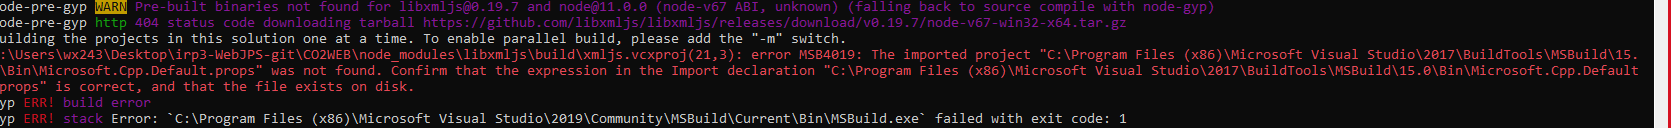
\includegraphics[scale=0.4]{error1.png}
    \label{fig:error1}
    \end{figure}
  \FloatBarrier
  The “Microsoft.Cpp.Default.props” was not found;
  Please check the folder mentioned in the error and make sure whether the aforementioned folder have this Microsoft.Cpp.Default.props file. If not, search this file. Then you’ll find its correct location and copy the path. If build tool 2019 is used, normally this file will be found in the path:
  C:$\backslash$Program Files (x86)$\backslash$Microsoft Visual Studio$\backslash$2019$\backslash$BuildTools$\backslash$MSBuild$\backslash$Microsoft$\backslash$VC$\backslash$v160$\backslash$.\\
  Then open environment variables and add a “VCTargetsPath” in both user variable and system veriables. The variable value is the path you find the “Microsoft.Cpp.Default.props” file and make sure the “ $\backslash$ “ is added at the end of the variable value.
  \FloatBarrier
    \begin{figure}[h!]
    \centering
    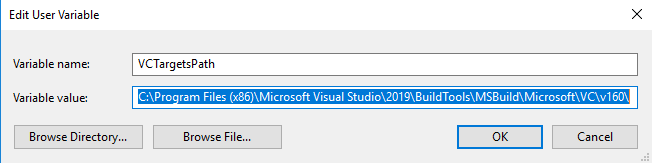
\includegraphics[scale=0.8]{vctargetspath.png}
    \label{fig:vctargetspath}
    \end{figure}
  \FloatBarrier  
  Also, to make the fellow setting-up run smoothly, please add new PATH to the environment variables: 
  \FloatBarrier
    \begin{figure}[h!]
    \centering
    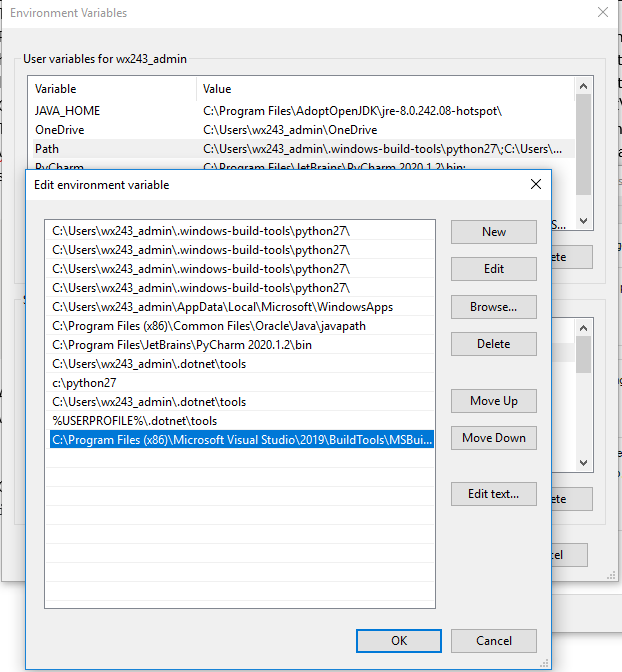
\includegraphics[scale=0.8]{path.png}
    \label{fig:path}
    \end{figure}
  \FloatBarrier 
  The whole path value is:\\ C:$\backslash$Program Files (x86)$\backslash$Microsoft Visual Studio$\backslash$2019$\backslash$BuildTools$\backslash$MSBuild$\backslash$Current$\backslash$Bin
  \\
  Once the environment variables are added, close the prompt window and reopen it. Try cmd: npm install again.\\
 \textbf{Error 2:}
  \FloatBarrier
    \begin{figure}[h!]
    \centering
    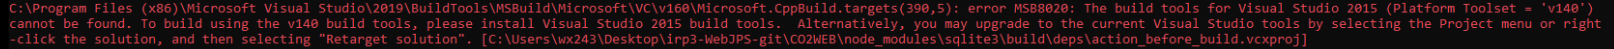
\includegraphics[scale=0.4]{error2.png}
    \label{fig:error2}
    \end{figure}
  \FloatBarrier  
 This error may arise when install package chokidar. Try this solution:\\
 \url{https://stackoverflow.com/questions/33154696/msbuild-error-the-builds-tools-for-v140-platform-toolset-v140-cannot-be-f}
 (But it may cause other errors that have not been solved yet).
 \item Download "redis-server":\\
 \url{https://github.com/dmajkic/redis/downloads?_ga=2.52270432.871911100.1594985060-965137043.1594985060}\\
 Unzip the file and open the folder 64bit. Doulbe click "redis-server.exe". 
 \item No matter what happen in Step 5, you can always run cmd: node app, to see if there is any other package that is needed to be installed. Just follow the instructions given when running node app until no farther packages needed to be added. 
 
\end{enumerate}
\end{document}
